\section{0-1 knapsack problem with volume extension}
In the last task the objective was to solve the adjusted Knapsack problem, where the knapsack is limited both by weight and volume limit. The Figure \ref{fig:knaspack_volume} shows the result of the algorithm terminating after 1000 iterations. It can be seen that after approximately 600 iterations the fitness function value does not change significantly.

\begin{figure}[!h]
	\centering
		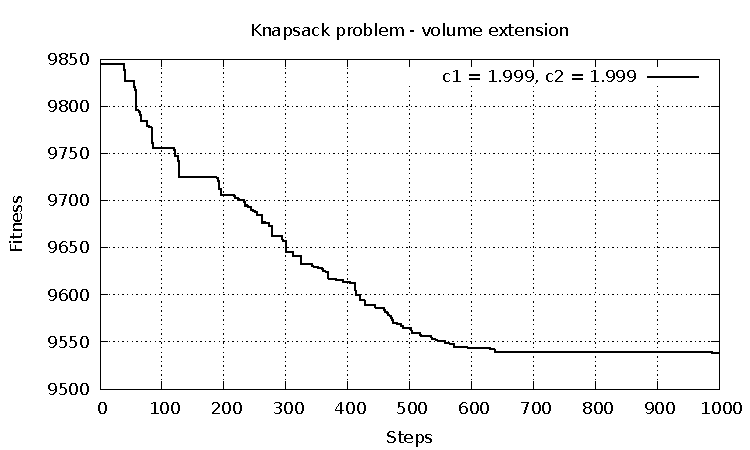
\includegraphics[width=15cm]{img/4a.pdf}
	\caption{Knapsack problem with the volume extension. The best gained the fitness function value of 9538, while filling the knapsack up to 997.2 kg and 962.3 $m^{3}$ with total value of 375. The second best result (dashed line) gained the fitness function value of 9841, while filling the knapsack up to 578.9 kg with total value of 72.0. The worst result (dotted line) gained the fitness function value of 9846, while filling the knapsack up to 585.47 kg with total value of 67.76.}
	\label{fig:knaspack_volume}
\end{figure}